%%%%%%%%%%%%%%%%%%%%%%%%%%%%%%%%%%%%%%%%%%%%%%%%%%
%%%%		~~~~ Literature ~~~~
%%%%%%%%%%%%%%%%%%%%%%%%%%%%%%%%%%%%%%%%%%%%%%%%%%


\chapter{Literature}
\label{chap:data}
\pagestyle{fancy}

The following section contains an extensive (though not exhaustive) categorical literature study. The first part provides contextual information, including motivations, and ethical concerns as well as a comprehensive overview of techniques used in music generation. The second half is more technical, with a discussion on music representation, tokenization, control and fine tuning. As a starting point, I used the most recent ISMIR (International Society for Music Information Retrieval) papers on music generation and their referenced sources, alongside other papers suggested by my advisor, Anja Volk. In addition, I performed systematic searches using the following keywords: Deep Learning Music Generation, Diffusion Music Generation, Transformer Music Generation, Symbolic Diffusion Music Generation, and Control Music Generation.

\section{Why Generate Music? - Motivation}
\subsection{Composition Co-Pilots}
The earliest music generators (including the 18th-century musical dice games\cite{Nierhaus_2009}) were justified as methods to inspire composers and music makers, including enabling novice composers to write music. Composer David Cope\cite{Cope_1989} states that he turned to music generation to overcome writer’s block. Commercial enterprises like Suno claim to be “building a future where everybody can make great music” \cite{Suno_AI}. Many current and past efforts highlight music generation as a process that assists composers. In DeepBach\cite{Hadjeres_Pachet_Nielsen_2017}, the authors go to great lengths to make the system flexible and usable in real-life composition scenarios. Initially, they developed a MuseScore integration and later tied DeepBach into the web app NONOTO\footnote{https://github.com/SonyCSLParis/music-inpainting-ts} to support musical inpainting in Ableton Live scores. Similarly, with Composer’s Assistant\cite{Malandro_2023}, the authors explicitly enable musical inpainting and continuation in the REAPER music production software. AI has also been explored as a co-improviser for live music-making, such as in Pachet's Continuator\cite{Pachet_2003} and Ben-Tal's musical dialog system\cite{Kite-Powell_2023}.

\subsection{Music in Games}
Beyond co-creating music, AI-generated music serves functional purposes, such as background music in videos and therapy-assisting games. In gaming, AI-generated or AI-assisted music is particularly relevant due to the scale and interactivity of games.

Video games often facilitate hundreds of hours of gameplay, featuring branching storylines and complex player interactions. However, game soundtracks typically cover only a fraction of that time\cite{Plut_Pasquier_2020, Worrall_Collins_2024}. Through different adaptive techniques, relatively short snippets of original material can be stretched into hours of unique audio, often relying on the recombination of different elements. However, rule-based recombination has its limitations. A recent study of player behavior \cite{Rogers_Weber_2019} finds that many players eventually turn off game music. They cite various reasons, such as preferring their own music over the game soundtrack (46.7\%) or finding the in-game music repetitive (29.6\%).

Procedural generation of 3D assets, levels, and enemy behavior is commonplace, but music generation remains underutilized. Composing and adapting music for every possible scenario would be tedious. AI-assisted music composition could enable adaptive audio on a large scale, either by creating numerous musical assets anticipating player choices or generating new variations of the game score in real time to enhance player immersion. However, several challenges make AI music generation difficult in games. Performance issues arise due to the resource-intensive nature of AI generators. Additionally, AI-generated music is difficult to control, and there is little guarantee that the generated tracks will be appropriate\cite{Plut_Pasquier_2020}. Furthermore, AI music generators currently lack proper integration into video game environments and engines\cite{Worrall_Collins_2024}.

\subsection{Music in Serious Games}
Aside from games for general audiences, generative music has potential applications in serious games. Serious games are designed for purposes beyond entertainment, such as education or therapeutic use, including music therapy\cite{Djaouti2011}. In music therapy, music can be used for emotion regulation, motivation, adherence, motor coordination, rhythmic entrainment, and facilitating social interactions\cite{musicwellbeing_agres_2021}. Musical attention control training has been shown to help individuals with Parkinson’s\cite{Park_Kim_2021}, ADHD\cite{Martin-Moratinos_Bella-Fernández_Blasco-Fontecilla_2023}, autism\cite{Pasiali_LaGasse_Penn_2014}, and psychosis\cite{van_Alphen_Stams_Hakvoort_2019} improve their mental capabilities for selective and switching attention. Serious games have the potential to supplement music therapy. “Last Minute Gig”\cite{Chalkiadakis_2022} implements clinical music therapy protocols as a serious game to improve attention control in Parkinson’s patients. However, users reported boredom and a lack of feedback, while more musically experienced users felt less challenged. Schlette\cite{Schlette_2022} attempted to address these issues by introducing dynamic difficulty adjustment through a feedback system alongside more complex music generation. This thesis aims to develop a controlled music generation model to improve player engagement through a richer music system.

\section{Why Not Generate Music? - Ethical Concerns} \label{ethical}
\subsection{Introduction}
There are several concerns related to AI-based music generation. First, there are legal concerns regarding copyright and licensing. Generative models may produce outputs that are identical or highly similar to copyrighted training data. Furthermore, the question remains whether models should be allowed to train on copyrighted data in the first place. Broader concerns include the devaluation of human labor and creativity, the oversaturation of cultural spaces with low-quality generated content, and the environmental impact of large generative models, which require substantial energy, water, and rare materials to operate.

\subsection{Data Leakage and Copyright}
Generative AI companies are achieving record-breaking valuations and this includes music generators with Suno at a valuation of about 500 million dollars after a 125  million dollar fund-raiser leading the pack. \cite{Stassen_2024} \cite{Tencer_2024}. However, AI companies are facing backlash from artists and record labels with an organization of record labels including the  “big three” Sony, Warner Music, and UMG suing Suno and Udio for \$150.000 dollars per infringed work\cite{Kaba_River_Perry_2024}.  Generative AI runs a substantial risk of parroting or leaking training data. In language models, the leakage problem is of concern when training on data that contains sensitive information, which may be revealed either through accidental leakage or through membership inference attacks \cite{Duan_Suri_Mireshghallah_Min_Shi_Zettlemoyer_Tsvetkov_Choi_Evans_Hajishirzi_2024}. While leakage may raise privacy concerns in other generative models such as speech and image-generators \cite{Carlini_Hayes_Nasr_Jagielski_Sehwag_Tramèr_Balle_Ippolito_Wallace_2023} for music, the risk of training data leakage is mostly an issue of copyright. Ed Newton Rex shows some examples of how Suno can be influenced \cite{Newton-Rex_2024} to leak training data. This ability to create disconcertingly close reproduction of copyrighted work is also cited in the court documents. Suno has since started to prevent prompting with artist names (i.e. in the style of Eminem) and including known song lyrics. 

\subsection{Training and Copyright}
Besides leaking training data, there is the more general question of whether AI models should be allowed to train on unlicensed work. Echoing the court case between OpenAI and the New York Times \cite{Reed_2024}, both Suno and Udio cite fair use in response to accusations of copyright infringement. In US copyright law the fair-use clause limits exclusive rights to a work, with four factors to consider: 1) purpose and character of the work in use, 2) nature of copyrighted work, 3) amount of the copyrighted work used, and 4) the effect on the potential market or value of copyrighted work.\cite{copyrightlaw}   Fair use is often granted to derivative works such as parodies and covers and works used in educational settings. AI’s learning of structures has also been likened to the human learning process, humans learn based on copyrighted music they listen to, without giving credit or compensation to their influences. Newton-Rex \cite{Newton-Rex_2024} rejects this comparison. In learning music, humans contribute to the musical ecosystem, they take lessons, go to performances, or at the very least generate some streaming revenue for artists, none of these are true for machine learning models learning from scraped data. 

\subsection{Devaluing Music}
While few are following director Ram Gopal Varma’s announcement to only use AI-generated music in his future films \cite{Singh_2024}, AI-generated music is becoming increasingly difficult to differentiate from human production and already receiving considerable amounts of streams and it is not unlikely that music in film, video and game projects may be replaced or at least supplemented with AI-generated music. The online music market is saturated, with more than 100,000 songs uploaded to music streaming giant Spotify every day \cite{Stassen_2023}. Generative AI may just further exacerbate this problem, resulting in a race to the bottom for creatives and musicians. 

\subsection{Environmental Impact}
Digital infrastructure, traditional data centers, crypto-currency mining, and AI-centered data infrastructure account for about 2\% of the world's energy consumption \cite{Marechal_2024}. The performance of current large language models often scales with simultaneous increases in model size, training data, and computation time.\cite{Kaplan_McCandlish_Henighan_Brown_Chess_Child_Gray_Radford_Wu_Amodei_2020}  Each of these three factors requires considerable resources. Music generation is no exception. In a recent ISMIR publication \cite{Holzapfel_Kaila_Jääskeläinen_2024} the authors make estimates on energy consumption of different projects related to music generation and computation-intensive MIR, finding an average energy consumption of 224.8kWh for model training (the energy consumption of an average western person over 2 months). The energy consumption is divided highly unevenly, with the median being at merely 18 kwh (3 days of an average westerner's energy consumption). Music generation models associated with large technology companies are responsible for about 89\% of the estimated energy use. This is only for training, models that are deployed publicly, continue to use substantial energy for inference. Beyond just the carbon footprint of generative AI, the local impacts of resource use such as rare minerals and water are important to keep in mind. 


\subsection{How  I plan to address these concerns}
During this thesis process, I’m planning to address the outlined ethical concerns in the following manner. First, I will only train, and use open-source models trained on licensed data providing attributions where possible. I will also make my trained models publicly available with substantial documentation to contribute to the open-source ecosystem, research, and music. Second I am explicitly designing the generative process to be cooperative, this is facilitated on the one hand through the introduction of new control modalities, and on the other the choice of symbolic music over audio, which eases editing and integration into composition software. Finally, I am not attempting to train custom large foundation models, rather I’m trying to find ways to extend existing models to introduce new control mechanisms, requiring training on only a fraction of the model parameters, with substantially less need for data, computation, and energy. 



\section{Overview of music generation}
From antique wind-chimes to classical period musical dice games to the aleatoric music of the 20th century - humans have used algorithmic, probabilistic, and statistical methods to create music. As early as the late 1940s, computers have played a role in composition as sound generators, instruments \cite{France-Presse_2016} and providing musical material themselves, such as in the 1957 Illiac suite \cite{Hiller_Isaacson_1959}. The following 50 years are characterized by disparate, academic experiments in music generation, mostly in the symbolic music domain. They utilize a variety of contemporary AI technologies, from expert systems and ontologies \cite{Hiller_Isaacson_1959}\cite{Ebcioğlu_1994} to evolutionary algorithms \cite{Polito_Daida_Bersano-Begey_1997} to feed-forward \cite{Todd_1989}, recursive \cite{Mozer_1994}, and convolutional neural networks \cite{coconet}. Some composers in the classical tradition, such as Iannis Xenakis \cite{Xenakis_1992} and David Cope\cite{Cope_1989} use computer algorithms in their creative work. 
In the 2010s a small ecosystem of commercial generative music startups such as Jukedeck, PopGun, and Ampermusic \cite{Featherstone_2017} starts to emerge, alongside an increasing number of publications applying deep learning, particularly Generative Adversarial Networks (GANs), and Recursive Neural Networks (RNN) to music including MIDInet \cite{midinet}, DeepBach \cite{Hadjeres_Pachet_Nielsen_2017} and FolkRNN \cite{Sturm_Ben-Tal_2016}. With the development of the transformer architecture in 2017 \cite{Vaswani_Shazeer_Parmar_Uszkoreit_Jones_Gomez_Kaiser_Polosukhin_2017}, large technology companies start experimenting with music generators including OpenAI’s Jukebox \cite{Dhariwal_Jun_Payne_Kim_Radford_Sutskever_2020} and Musenet\cite{Christine_2019}, Meta’s MusicGen\cite{copet2023simple} and Google’s MusicLM \cite{Agostinelli_Denk_Borsos_Engel_Verzetti_Caillon_Huang_Jansen_Roberts_Tagliasacchi_et_al._2023} and the preceding Magenta project, with fully generative models capable of producing sequences of high-quality music modeled from raw audio. At the time of writing, commercial music generators such as Suno and Udio are raising millions of dollars in investment funds\cite{Stassen_2024}, while generated music is being widely streamed and actively used in TV and video productions. 

\section{Non-neural music generation}

\subsection{Why look beyond deep learning}
Neural, specifically deep learning (DL) systems, currently receive considerable attention. However, given their substantial drawbacks relating to explainability, transparency, computational efficiency, copyright and licensing issues, and their enormous need for data (more in section \ref{ethical}), it is worthwhile considering alternative approaches to music generation. A recent study \cite{Yin_Reuben_Stepney_Collins_2023} performs a comprehensive listening survey comparing neural net and non-neural net systems. The top-performing systems a Markov Model -  MAIA Markov \cite{Collins_Laney_2017}  and a deep learning system  - MusicTransformer \cite{Huang_Vaswani_Uszkoreit_Shazeer_Simon_Hawthorne_Dai_Hoffman_Dinculescu_Eck_2018} perform similarly well in the listening study. The choice of one of the earliest transformer-based music from 2018 \cite{Huang_Vaswani_Uszkoreit_Shazeer_Simon_Hawthorne_Dai_Hoffman_Dinculescu_Eck_2018} and the restriction to symbolic music, raises questions, whether their conclusion of similar performance still holds. Considering the study was published in 2023, these are important limitations. However, their criticism that many DL-based music generation projects do not look beyond DL and compare their systems based on technical metrics - with no obvious impact on how human listeners perceive the output remains solid. Finally, many hybrid approaches successfully combine traditional rule-based or statistical methods with deep learning. Those methods may help researchers and developers maintain a more comprehensive toolkit of techniques and paradigms. 

\subsection{Rule-based music generation}
Non-neural net systems can classified as either rule-based or statistical. Both types have been part of some of the earliest attempts at music generation. Centuries of style-defining musicological writing from ancient Mesopotamian tuning charts \cite{Mirelman_2013} to Fux`s Gradus ad Parnassum \cite{Fux_1725} and Arnold Schönberg`s 12-tone music have crystallized sets of rules that approximate various styles of music. Many approaches to music generation take advantage of this knowledge and codify it into a computer program, creating expert systems for music generation. In Hiller \& Isaacson`s Illiac Suite, a series of experimental, computational compositions, the first and second movements are generated following the rules of first species counterpoint \cite{Fux_1725}, approximating Palestrina's contrapuntal technique. Some rules aim to contain the melody, such as limiting the range to an octave, enforcing the identical start and end notes, and avoiding consecutive melodic jumps. Other rules aim to constrain harmony, such as forbidding parallel octave, fifth, and fourth motion and enforcing consonant harmonies. Hiller and Issacson's approach is relatively simple, using only a handful of conditions (see figure \ref{fig:hillerissacson}). Rule-based generation can be highly complex, such as CHORAL \cite{Ebcioğlu_1994} (for which the developer also built a custom programming language), which encodes over 300 rules to realize bach-style chorales from a given melody. 

\begin{figure}[H]
    \centering
    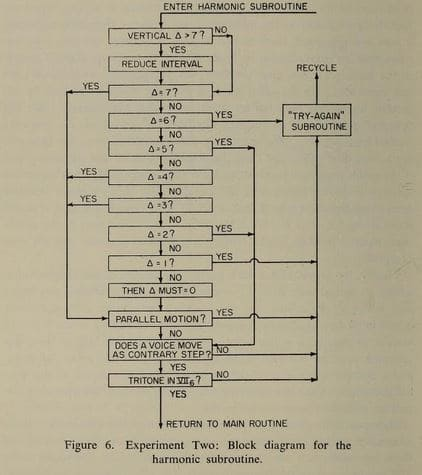
\includegraphics[width=0.5\textwidth]{IMAGES/IlliacRuleBased.jpg} 
    \caption{Rule-Based - Block Diagram from Hiller and Issacson’s book  - explaining movement two of the 1957 Illiac Suite. }
    \label{fig:hillerissacson}
\end{figure}

\subsection{Markov Model Music Generation}
Markov models remain a popular method of generating music to this day. At its simplest, a Markov music generator could work off of a transition matrix for pitch classes, such as Richard Pinkerton’s 1956 “Banal Melody Generator” \cite{Pinkerton_1956}. 
Markov chains can be nested or constrained for more complex interactions \cite{Collins_Laney_2017}. In Hiller and Isaacson's \cite{Hiller_Isaacson_1959} fourth movement of the Illiac suite, they use Markov chains with a table of possible intervals stretching from unison to octave. In the latter sections of the movement, they introduce additional restrictions to add memory to the method through higher-order Markov chains that reference previously generated music. 
Transition matrices can be built from very little data, such as short improvisations \cite{Pachet_2003}, but training over a whole corpus is also viable. Other systems configure Markov chains to take additional inputs into account, such as Allan, \cite{Allan_2002} who generates harmonies to given melodies in the style of Bach. This makes Markov model-based systems very flexible and relatively lightweight.

\begin{figure}[H]
    \centering
    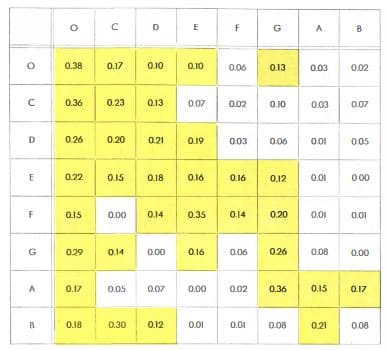
\includegraphics[width=0.5\textwidth]{IMAGES/PinkertonNurseryRhymes.jpg} 
    \caption{Transition matrix from Pinkerton's 1956 “Banal Music Generator”. Probability of a pitch (row) following on a pitch (column), likely pairs are marked in yellow. The probabilities are calculated from a set of 39 nursery rhymes.}
    \label{fig:pinkertonmatrix}
\end{figure}\subsection{Other statistical approaches}
Music generation has also been attempted with other means, such as metaheuristic search for harmony or melody \cite{Altay_Alatas_2018}. In Morpheus, \cite{Herremans_Chew_Morpheus_2019} the developers use variable neighborhood search (VNS) to generate polyphonic pieces following a tension profile for long-term structure. Closely related to this approach are evolutionary and genetic algorithms such as Politio et al's \cite{Polito_Daida_Bersano-Begey_1997} model of 16th-century counterpoint as a multi-population problem. Here, three separate populations of agents generate instructions focusing on different musical aspects, such as harmony or imitation, and are evaluated based on individual performance and symbiotic performance together with the other agents over multiple generations. 


\subsection{Early Neural Net based systems}

Music generators based on neural nets were introduced as early as 1989. Todd et al. \cite{Todd_1989} generate melodies using a fixed window for a conventional feed-forward neural network but also introduce a feedback loop feeding the network's previous state to the next iteration. Future work based on RNNs uses the latter principle, such as CONCERT,\cite{Mozer_1994} a 1994 RNN trained to generate melodies based on datasets of Bach chorales, waltzes, and European folk songs. There are also hybrid systems such as HARMONET \cite{Hild_Feulner_Menzel_1991}, an RNN-based music generator for re-harmonizing Bach chorales. It merges the RNN with a symbolic rule-checking algorithm. More recent RNN-based music generators, such as FolkRNN \cite{Sturm_Ben-Tal_2016}, a melody generator trained on Irish folk songs, use long short-term memory (LSTMs) or gated recurrent units (GRUs). Generative Adversarial Networks (GANs) and Variational Autoencoders (VAEs) remain popular architectures for music generation. \cite{Civit_Civit-Masot_Cuadrado_Escalona_2022}

\section{Deep learning for music generation}
State-of-the-art music generation, including many commercial applications, leverages the advances in language and image generation over the last five years. Two distinct approaches, namely autoregressive, transformer-based, and diffusion-based approaches dominate.


\subsection{Transformers - sequence modeling without recurrence}
Autoregressive music generation draws from successful natural language modeling tasks powered by the transformer model. Transformers were originally developed for the task of language translation.\cite{Vaswani_Shazeer_Parmar_Uszkoreit_Jones_Gomez_Kaiser_Polosukhin_2017} They keep the self-attention mechanism already deployed in LSTMs for seq2seq tasks \cite{Sutskever_Vinyals_Le_2014} but replace the recurrent connection with positional embeddings and masked attention. This allows the model to train on all tokens in parallel instead of one token at a time, which enables much larger and more capable models trained at a fraction of the time required to train similarly large RNNs. The transformer comes in several different configurations. The original transformer contains encoder and decoder layers - see figure \ref{fig:transformer}. Often, tasks relating to sequence understanding, such as music classification, use an encoder-only architecture. The BERT series of language models \cite{Devlin_Chang_Lee_ToutanovaBERT_2019} and music understanding models such as MusicBERT\cite{Zeng_Tan_Wang_MUSICBERT_2021} are examples. 
On the other hand, sequence generation tasks often employ a decoder-only architecture, this includes the GPT-series \cite{Radford_Wu_Child_Luan_gpt2_2019} and many music generators such as MusicGen\cite{copet2023simple}. The transformer architecture is the baseline for all current large language models. Transformers are used in modalities beyond text, including images, audio, or DNA sequences.

\begin{figure}[H]
    \centering
    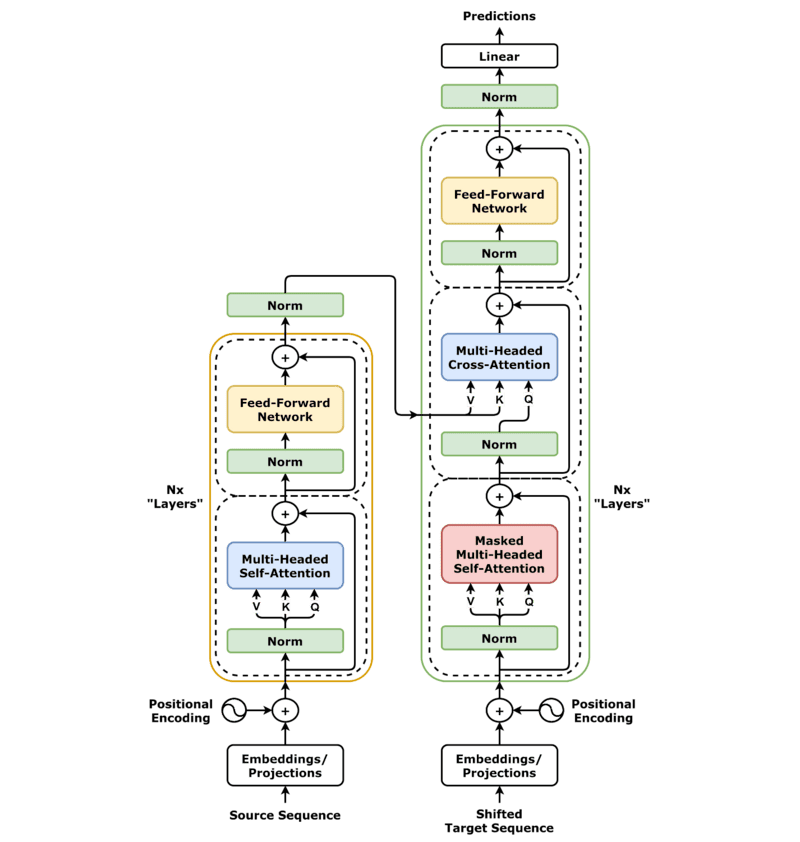
\includegraphics[width=0.5\textwidth]{IMAGES/Transformer,_full_architecture.png} 
    \caption{Schema of the full transformer encoder-decoder architecture}
    \small\textsuperscript{a=} By dvgodoy - CC BY 4.0, https://commons.wikimedia.org/w/index.php?curid=151216016
    \label{fig:transformer}
    
\end{figure}

\subsection{Diffusion models - spectrograms and piano-rolls}
Diffusion models are widely used for image and audio generation. Diffusion models learn to remove noise from a distribution (i.e. an image). Random noise is added to an image, and the model learns to undo this addition. During inference, the model starts with random noise (often accompanied by a guiding text prompt) and undoes it until it arrives at a clear image. AudioLDM \cite{Liu_Chen_Yuan_Mei_Liu_Mandic_Wang_Plumbley_2023}, and StableAudio \cite{Evans_Parker_Carr_Zukowski_Taylor_Pons_2024} are diffusion models that operate based on continuous audio encoding by a variational autoencoder. Diffusion models have also been used to generate symbolic music. Polyffusion \cite{Min_Jiang_Xia_Zhao_polyffusion_2023} uses image representations of piano rolls and adapts their diffusion model for various tasks, inpainting, accompaniment, and melody generation and generation based on a given chord sequence or texture. 

In this thesis, we will be targeting transformer models. Transformer models are tremendously popular and behind many state-of-the-art results in music generation. There is a tremendous amount of interest in model fine-tuning and control. In addition, many efforts aim to efficiently adjust models to related tasks without going through the relatively costly training procedure of large models. There is a large selection of open-source models that generate music and excellent infrastructure to support the training and evaluation of those models. 

\section{Representation and Format}\label{representation}
The choice of representation of data is a crucial aspect of music generation. First, the choice of audio or symbolic music has consequences for data availability, dataset size, context of the output, and what features can be controlled. Second, tokenization, the method in which symbolic or audio data are chunked and ingested into the model is an important aspect, with tradeoffs to consider for different generative tasks and goals. 


\subsection{Symbolic Music vs Audio}
Music can be represented digitally in two ways, either as an audio rendition or symbolically as a set of instructions. Working with different representations comes with various drawbacks and benefits for music generation. There are different types of symbolic representations of music, but the most common consist of discrete sequences of musical elements such as pitch or duration.  Working with audio theoretically gives access to all audible qualities of music, including detailed information on instrumental timbre or acoustic settings. In symbolic music, this is restricted to pitch, duration, and instrumentation, which sometimes is extended to include formatting information such as bar lines, etc. 
Symbolic data is also far less available than audio data. Many symbolic music datasets are created by compiling hand-transcribed music. High-quality automatic transcription remains an unsolved issue.\cite{Ji_Yang_Luo_survey_symbolic_2024}\cite{Chen_Smith_Spijkervet_Wang_Zou_Li_Kong_Du_2024}  However, symbolic music gives more direct access to many higher-level musical features such as chord progressions, melodies, and instrumentation. When working with audio, these features have to be extracted first, requiring additional processing steps that are prone to inaccuracies. 
Another consideration to take into account is size. Raw audio is significantly larger than a corresponding digital score. In addition, rendered audio is difficult to edit once generated. 

\subsection{Tokenisation}
Sequences are typically transformed into tokens, a numerical representation of data, to be handled by a machine learning algorithm. Audio-based music generation uses tokenization to condense audio while retaining its semantic content. Jukebox \cite{Dhariwal_Jun_Payne_Kim_Radford_Sutskever_2020} uses a variational autoencoder\cite{Kingma_Welling_2014} with a discretizing bottleneck (VQ-VAE) to create tokens from audio. Musicgen \cite{copet2023simple} tokenizes audio using the previously developed Encodec model for audio compression which similarly to VQ-VAE, learns a highly condensed discrete representation of audio \cite{Défossez_2023_encodec}. These condensed encodings are crucial for generative modeling on audio.

\subsection{Symbolic Tokenisation} \label{symbolic tok}
Due to its discrete representation, symbolic music is typically not condensed further (with some notable exceptions, such as condensed piano roll representation for symbolic music diffusion \cite{Min_Jiang_Xia_Zhao_polyffusion_2023}\cite{Zhu_Liu_Jiang_Zheng_texture_2024}). However, the choice of tokenization influences the model's performance on different music generation tasks. \cite{Fradet_Briot_Chhel_2021}. Common ways of tokenizing symbolic music align closely with the musical instrument digital interface (MIDI) standard, with individual tokens encoding different midi-events such as note-on, note-off, and velocity. The REMI+ \cite{Huang_Yang_remi_pop_transformer_2020} tokenization expands on MIDI-based tokenization with tokens for bar and position, designed to help capture recurring musical patterns. The PerTok tokenizer designed by Lemonaid\footnote{https://www.lemonaide.ai/}  encodes micro timings and offsets, designed to capture the full spectrum of rhythm in musical performances.

These extensions come at a cost: The resulting sequences can become very long, which adversely affects the model\cite{Ji_Yang_Luo_survey_symbolic_2024}. Ongoing attempts are made to condense token sequences, such as compound words or nested tokens.\cite{Ryu_Dong_nested_2024}. Dong et al.\cite{Dong_Chen_MMT_Kirkpatrick_2023} combine six different MIDI-like events (type, beat, position, pitch, duration, instrument) into single tokens. Hsiao et al.\cite{compound_word_Hsiao_Liu_Yeh_Yang_2021} differentiate between token types and group neighboring tokens into compound words, resulting in significantly shorter sequences (about 50\% compared to individual tokens). 

This thesis uses a third approach: Byte Pair Encoding (BPE) \cite{Sennrich_Haddow_Birch_BPE_2016}. BPE is used widely in language modeling, including the GPT series of models\cite{Radford_Wu_Child_Luan_gpt2_2019} and has been successfully applied to symbolic music generation.\cite{Fradet_Gutowski_Chhel_Briot_2023} The approach is simple: the most common token-pairs of the dataset are repeatidly combined into new combined tokens until the total amount of unique tokens reaches a preset vocabulary size. This approach works independently of token types and semantic content of the tokens and allows for very flexible scaling of the vocabulary. As seen in figure \ref{fig:tok_compare}, this drastically shortens the sequence length by about a third ($mean_{individual}=47976, mean_{bpe}=14519$), which in turn improves both the quality and efficiency of the model. 

\begin{figure}[H]
    \centering
    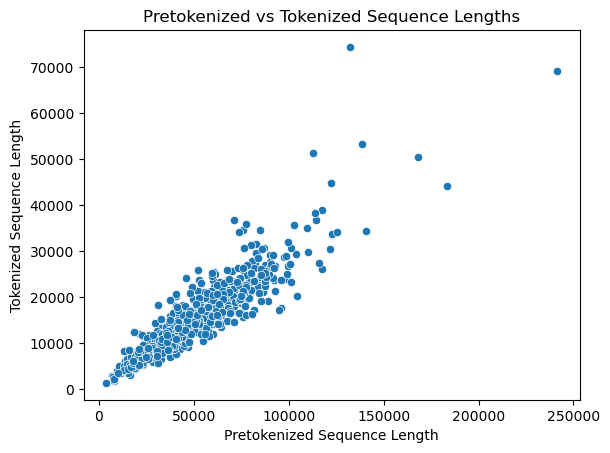
\includegraphics[width=0.5\textwidth]{IMAGES/scatter_pre_post_tok.png} 
    \caption{Scatterplot of individual vs bpe-tokenization sequence lengths}
    \label{fig:tok_compare}
\end{figure}



See table \ref{table:bigtable} in the appendix for a more elaborate display of representations used in symbolic music generators

\cite{Herremans_Chew_Morpheus_2019} 

\section{Deep Learning and Symbolic Music Generation}
Various approaches to symbolic music generation use deep learning. However, there are considerable differences in the implementation, such as choice of architecture and representation, that influence the model's capabilities, use case, and what aspects the user can control. The following table summarizes these key characteristics across a selection of approaches that inspire our model. For a comprehensive survey of representation, tasks, and evaluation methods used in symbolic deep learning music generation see \cite{Ji_Yang_Luo_survey_symbolic_2024}.

\begin{table}[H] \label{table:bigtable}
    \centering
    \renewcommand{\arraystretch}{1.2} % Adjust row height
    \setlength{\tabcolsep}{3pt} % Adjust column spacing
    \scriptsize % Set smaller font size
    \begin{tabular}{|p{2.5cm}|p{1.8cm}|p{3cm}|p{1cm}|p{1cm}|p{3cm}|p{2.5cm}|}
        \hline
        \textbf{Name} & \textbf{Architecture} & \textbf{Control} & \textbf{TV} & \textbf{MI} & \textbf{Dataset} & \textbf{Representation} \\
        \hline
        FolkRNN 2015 \cite{Sturm_Ben-Tal_2016} & RNN & meter, mode & No & No & TheSession \cite{sessionfolkdata} & REMI-Like\\
        DeepBach 2017 \cite{Hadjeres_Pachet_Nielsen_2017} & RNN & Inpainting & Yes & Yes & JSB-chorales \cite{jsbchorales} & Midi-Like\\ 
        MusicTransformer (2018) \cite{Huang_Vaswani_Uszkoreit_Shazeer_Simon_Hawthorne_Dai_Hoffman_Dinculescu_Eck_2018} & Transformer & - & No & No & Maestro \cite{hawthorne2018maestro},  JSB-chorales\cite{jsbchorales} & Midi-Like\\
        MuseNet 2019 \cite{Christine_2019} & Transformer & instrument, genre & Yes & Yes & Mastro \cite{hawthorne2018maestro}, CX \cite{classicalarchives}, BM \cite{bitmidi} & ?\\
        MidiNet 2019 \cite{midinet} & GAN & chords, melody & Yes & Yes & HTPM \cite{hooktheorypopmidi} & Midi-Like\\
        Fader Nets 2020\cite{Tan_Herremans_2020} & VAE & arousal & No & No & Maestro \cite{hawthorne2018maestro} & Custom \\
        MMM 2020 \cite{Ens_Pasquier_2020_MMM} & Transformer & inpainting, instrument, note-density & Yes & Yes & Lakh MIDI \cite{Raffel_2016} & MMM\\
        PopTransformer 2020 \cite{Huang_Yang_remi_pop_transformer_2020} & Transformer & chords, tempo & Yes & No & Custom & REMI\\
        Museformer 2022 \cite{Yu_Lu_Wang_Hu_Tan_Ye_Zhang_museformer_2022} & Transformer & - & No & Yes & LakhMIDI \cite{Raffel_2016} & REMI-Like\\
        Polyfussion 2023 \cite{Min_Jiang_Xia_Zhao_polyffusion_2023} & Diffusion & inpainting, texture & Yes & No & POP90 \cite{Wang_Chen_pop90_dataset} & Piano-Roll\\
        FIGARO 2023 \cite{Rütte_figaro_2023} & Transformer & chords, instrument, meter, note-density & Yes & Yes & Lakh MIDI \cite{Raffel_2016} & REMI+ \\
        MMT 2023 \cite{Dong_Chen_MMT_Kirkpatrick_2023} & Transformer & instrumentation & No & Yes & Lakh MIDI \cite{Raffel_2016}, SOD \cite{Crestel_OrchestralDataset} & Midi-Tuple \\
        Sympack 2024 \cite{Chen_Smith_Spijkervet_Wang_Zou_Li_Kong_Du_2024} & Transformer & chords, structure, notes & Yes & Yes & Lakh MIDI\cite{Raffel_2016}, \cite{Bertin-Mahieux_Ellis_Whitman_Lamere_2011}, Custom & -\\
        MuseCoco 2023 \cite{Lu_Xu_Kang_Yu_Xing_Tan_Bian_MuseCoco_2023} & Transformer & Genre, tempo, emotion ...  & No & No & Custom & REMI-Like\\
        MuseBarControl 2024 \cite{Shu_Xu_Musebarcontrol_2024} & Transformer & chords & Yes & No & POP90 \cite{Wang_Chen_pop90_dataset} & REMI-Like\\
        NTT 2024 \cite{Ryu_Dong_nested_2024} & Transformer & - & No  & Yes & Lakh MIDI \cite{Raffel_2016}, POP90 \cite{Wang_Chen_pop90_dataset}, SOD \cite{Crestel_OrchestralDataset} & Compound\\
        FTG 2024 \cite{Zhu_Liu_Jiang_Zheng_texture_2024} & Diffusion & texture, rhythm, chords & Yes & No & POP90 \cite{Wang_Chen_pop90_dataset} & Piano-Roll \\
        NDRD 2024 \cite{Huang_rule_diffusion_2024} & Diffusion & chord, pitch, note-density & Yes & No & Maestro \cite{hawthorne2018maestro}, POP90 \cite{Wang_Chen_pop90_dataset} & Piano-Roll \\
        \hline
    \end{tabular}
    \caption{Overview of symbolic, deep learning based music generation models, their architectures, and control mechanisms, time-vayring control (TV), multitrack capabilities (MI), dataset, and representation. A more complete Overview
    is found in \cite{Ji_Yang_Luo_survey_symbolic_2024}}
    \label{tab:music_models}
\end{table}

\section{Representation and Format}\label{section:representation}
The choice of representation of data is a crucial aspect of music generation. First, the choice of audio or symbolic music has consequences for data availability, dataset size, context of the output, and what features can be controlled. Second, tokenization, the method in which symbolic or audio data are chunked, organized, and ingested into the model is an important aspect, with tradeoffs to consider for different generative tasks and goals. 


\subsection{Symbolic Music vs Audio}\label{section:symbolic_audio}
Music can be represented digitally in two ways, either as an audio rendition or symbolically as a set of instructions. Working with different representations comes with various drawbacks and benefits for music generation. There are different types of symbolic representations of music, but the most common consists of discrete sequences of musical elements such as pitch or duration.  Working with audio theoretically gives access to all audible qualities of music, including detailed information on instrumental timbre or acoustic settings. In symbolic music, this is more restricted. 

Symbolic data is also far less available than audio data. Many symbolic music datasets are created by compiling hand-transcribed music. High-quality automatic transcription remains an unsolved issue.\cite{Ji_Yang_Luo_survey_symbolic_2024}\cite{Chen_Smith_Spijkervet_Wang_Zou_Li_Kong_Du_2024}. This is a serious limiting factor on how large symbolic music generators can become. However, symbolic music gives more direct access to many higher-level musical features such as chord progressions, melodies, and instrumentation. When working with audio, these features have to be extracted first, requiring additional processing steps that are prone to inaccuracies. 
Another consideration to account for is size: raw audio is significantly larger than a corresponding digital score. In addition, rendered audio is difficult to edit once generated. 
 
\subsection{Tokenisation}\label{section:tokenization}
Sequences are typically transformed into tokens, a numerical representation of data, to be handled by a machine learning algorithm. Audio-based music generation uses tokenization to condense audio while retaining its semantic content. Jukebox \cite{Dhariwal_Jun_Payne_Kim_Radford_Sutskever_2020} uses a variational autoencoder\cite{Kingma_Welling_2014} with a discretizing bottleneck (VQ-VAE) to create tokens from audio. Musicgen \cite{copet2023simple} tokenizes audio using the previously developed Encodec model for audio compression which, similarly to VQ-VAE, learns a highly condensed discrete representation of audio \cite{Défossez_2023_encodec}. These condensed encodings are crucial for generative modeling on audio. Depending on the representation, a similar technique is used to encode piano rolls for diffusion of symbolic music \cite{Min_Jiang_Xia_Zhao_polyffusion_2023}\cite{Zhu_Liu_Jiang_Zheng_texture_2024}.

\subsection{Symbolic Tokenisation} \label{section:symbolic_tok}
Symbolic music is represented is in different ways, such as text (i.e. the ABC notation), piano roll, graph, and sequences. The most widely used representation, however, is the event-based MIDI representation, which is reflected in the tokenization techniques. In symbolic music, tokenizers are feature extractors. They extend the standard MIDI vocabulary with additional tokens that help models better capture different aspects of music.\cite{Fradet_Briot_Chhel_2021}. In table \ref{table:bigtable} the tokenization approach of different symbolic models is summarized.\\
\textbf{MIDI-Like} tokenization closely emulates the MIDI vocabulary, translating a MIDI file into a single stream of tokens such as note-on and note-off. The \textbf{MMM} tokenizer adds indicators to aid track-inpainting. \textbf{REMI} \cite{Huang_Yang_remi_pop_transformer_2020} tokenization expands on MIDI-based tokenization with tokens for duration, bar, and position, designed to help capture recurring musical patterns. \textbf{REMI+} \cite{Rütte_figaro_2023} tokenization extends \textbf{REMI} with an instrument token to better encode multi-instrument tracks. The \textbf{PerTok} tokenizer designed by Lemonaid\footnote{https://www.lemonaide.ai/}  encodes micro timings and offsets designed to capture the full spectrum of rhythm in musical performances.\\

These extensions come at a cost: The resulting sequences of tokens can become very long, which adversely affects the model \cite{Ji_Yang_Luo_survey_symbolic_2024}. Ongoing attempts such as compound word or nested tokens aim to shorten the sequences by combining low-level tokens into more expressive high-level tokens.\cite{Ryu_Dong_nested_2024}. Dong et al.\cite{Dong_Chen_MMT_Kirkpatrick_2023} combine six different MIDI-like events (type, beat, position, pitch, duration, instrument) into single tokens. Hsiao et al.\cite{compound_word_Hsiao_Liu_Yeh_Yang_2021} differentiate between token types and group neighboring tokens into compound words, resulting in significantly shorter sequences (about 50\% compared to individual tokens). 

This thesis uses a third approach: Byte Pair Encoding (BPE) \cite{Sennrich_Haddow_Birch_BPE_2016}. BPE is used widely in language modeling, including the GPT series of models\cite{Radford_Wu_Child_Luan_gpt2_2019} and has been successfully applied to symbolic music generation.\cite{Fradet_Gutowski_Chhel_Briot_2023} The approach is simple: the most common token pairs of the dataset are repeatedly combined into new combined tokens until the total amount of unique tokens reaches a preset vocabulary size. This approach works independently of token types and semantic content of the tokens and allows for very flexible scaling of the vocabulary. As seen in figure \ref{fig:tok_compare}, this drastically shortens the sequence length by about a third ($mean_{individual}=47976, mean_{bpe}=14519$), which in turn improves both the quality and efficiency of the model. 


\begin{figure}[H]
    \centering
    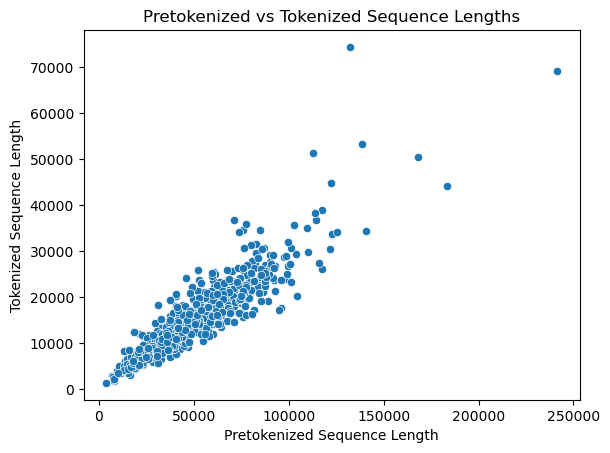
\includegraphics[width=0.5\textwidth]{IMAGES/scatter_pre_post_tok.png} 
    \caption{Scatterplot of sequence length before and after BPE tokenisation}
    \label{fig:tok_compare}
\end{figure}
\section{Control} \label{section:control}
Control is an essential aspect of any generative model. Without control, even the best generative models producing beautiful music are of limited real-world use. Control allows generative AI tools to become proper collaborative systems, which generate for a wide array of scenarios. In music generation, control covers essentially all musical features. Available features vary by representation. To illustrate:
Raw audio models such as Stable Audio (Evans et al., 2024) can be controlled for acoustic settings (i.e jazz music playing in a \textit{busy restaurant}, in a \textit{large cathedral}, or \textit{through an intercom}), something that is simply not represented in symbolic music. 

There are different approaches to classifying musical features. 
One can differentiate between global and local features (discussed in the appendix \ref{feature_cat}) \cite{Van_Kranenburg_Volk_Wiering_2013}, 
deep vs surface-level features \cite{Blacking_1971}, high-level versuss low-level features \cite{Tan_Herremans_2020} and global versus fine-grained or time-varying features. 

In the context of this thesis, we differentiate between global features and time-varying features \cite{Rütte_figaro_2023}. Global features as features that do not change within an excerpt, while time-varying features can change within an excerpt. What is time-varying or global is highly context-dependent, a piece may have a single time time-signature and tempo as is assumed in \cite{Lu_Xu_Kang_Yu_Xing_Tan_Bian_MuseCoco_2023} or it may vary throughout the piece as enabled in \cite{Rütte_figaro_2023} or \cite{Huang_Yang_remi_pop_transformer_2020}. Other time varying controls could be chords \cite{Rütte_figaro_2023}\cite{Wu_Donahue_musicontrolnet_2023}\cite{Lan_Hsiao_Cheng_Yang_musicongen_2024}\cite{Min_Jiang_Xia_Zhao_polyffusion_2023}, melody \cite{copet2023simple}\cite{Min_Jiang_Xia_Zhao_polyffusion_2023} or texture \cite{Min_Jiang_Xia_Zhao_polyffusion_2023}. For the target application in a MACT - game, time-varying controls are necessary to provide a change in music that triggers a change in the patient's improvisation. See table \ref{table:bigtable} for an overview of what features are controlled for, and whether they are time varying or not. 


\subsection{Rhythmic control} \label{section:rhytmic_weight}
The types of control exercised over rhythmic components vary by representation as discussed in \ref{representation}. In CocoMulla \cite{Lin_cocomulla_2024} generated audio is controlled with drum tracks and a piano roll. Similarly, in JASCO\cite{Tal_jasco} drum audio is used for conditioning. In MusicConGen \cite{Lan_Hsiao_Cheng_Yang_musicongen_2024}, control for rhythm is added through tracking beats and downbeat. MusicControlNet\cite{Wu_Donahue_musicontrolnet_2023} adds beat and downbeat conditioning to an audio diffusion model.
For symbolic systems, control of tempo and meter is relatively common \cite{Rütte_figaro_2023}, \cite{Huang_Yang_remi_pop_transformer_2020}, \cite{Lu_Xu_Kang_Yu_Xing_Tan_Bian_MuseCoco_2023}. Time-varying control over rhythm is often deployed through note density (both vertical and horizontal)\cite{Rütte_figaro_2023},\cite{Huang_rule_diffusion_2024}. Another approach \cite{Zhu_Liu_Jiang_Zheng_texture_2024} involves passing the piano roll as a factor to guide the diffusion process. In Polyffusion\cite{Min_Jiang_Xia_Zhao_polyffusion_2023} Min et al. successfully encode texture that is disentangled into harmony and rhythm using a pre-trained variational auto-encoder \cite{Wang_vae_chord_rhythm_2020}. Herremans et al. \cite{Tan_Herremans_2020} control rhythm through the high-level feature arousal, which they disentangle into rhythm and note density using a variational autoencoder. 

\subsection{Inner Metric Analysis} 
We could use a variational auto-encoder to disentangle rhythmic descriptions into lower-level features. However, it introduces the additional complexity of training a second model and using it for inference. Instead, we investigate Inner Metric Analysis (IMA) for its potential to control the rhythm of a generated excerpt over time. Inner Metric Analysis identifies strong and weak pulses and their periods within note onsets in symbolic music. It is used to identify \textit{local meters} as opposed to \textit{outer meter} given by time-signatures, which can be useful in the study of syncopation \cite{Bemman2024}\cite{Volk2008Syncopation}. IMA is also used in the classification of dance-music \cite{Chew_Volk_Lee_Dance_metric_weight_2005}, automatic detection of meter \cite{Haas_Volk_2016} and music retrieval \cite{Volk_Garbers_VanKranenburg_Wiering_Grijp_Veltkamp_2009}. 

A local meter is a set of evenly spaced onsets with a minimum length of three, not able to be extended forward or backward in time, and not contained within any other local meter. (see figure \ref{fig:ima_all}). Let $M(l)$ be the set of local meters with a length of at least l. The parameter $p$ is variable and determines how much the length of a local meter influences its weight. Intuitively, longer and more established local meters should carry more weight. This is given by $k_{m}^p$. The weight of an onset $W_{l,p}(o)$ is defined as the weighted sum of the local meters.  
The metric weight is calculated as follows \cite{Volk2008Syncopation}.  

\begin{equation}
 W_{l,p}(o) = \sum_{m \in M(l):o \in m}k_{m}^{p}
\end{equation} 
Spectral weight is a variation of metric weight, that considers the extension of each local meter: $ext(m)$. The red triangles in figure \ref{fig:ima_all} are an example of extensions. The calculation is similar, but it assigns a weight to each time point (instead of only to onsets) and considers the extensions. This feature is less sensitive to local changes.

\begin{equation}
 SW_{l,p}(t) = \sum_{m \in M(l):t \in ext(m)}k_{m}^{p}
\end{equation}

IMA can indicate rhythmic complexity. This, in turn, influences the ease of tapping along/following \cite{Volk2008Syncopation} and rhythmic entrainment. Configured properly, IMA could be utilized to generate music that is more difficult to follow, allowing for difficulty adjustment in the context of a MACT game. 


\begin{figure}[H]
    \centering
    \begin{subfigure}{0.45\textwidth}
        \centering
        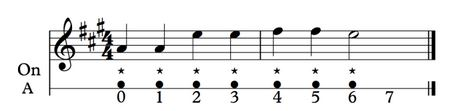
\includegraphics[width=\linewidth]{IMAGES/IMA1.JPG}
        \caption{Single local meter and its pulses (A) from the melody "Twinkle, Twinkle Little Star"}
        \label{fig:ima1}
    \end{subfigure}
    \begin{subfigure}{0.45\textwidth}
        \centering
        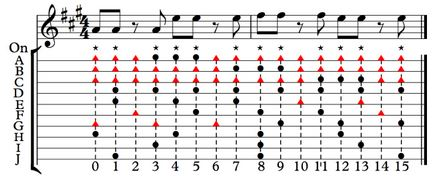
\includegraphics[width=\linewidth]{IMAGES/IMA2.JPG}
        \caption{10 local meters and their pulses produced by IMA of a syncopated variation of "Twinkle, Twinkle Little Star"}
        \label{fig:ima2}
    \end{subfigure}
    
    \vspace{0.5cm} % Adjust spacing between rows

    \begin{subfigure}{0.45\textwidth}
        \centering
        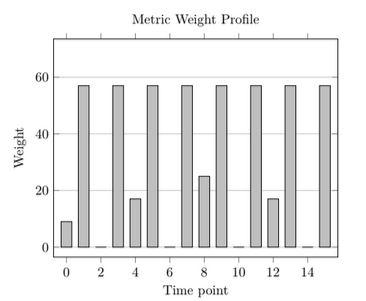
\includegraphics[width=\linewidth]{IMAGES/IMA3.JPG}
        \caption{Metric weight profile of syncopated "Twinkle, Twinkle Little Star"}
        \label{fig:ima3}
    \end{subfigure}
    \begin{subfigure}{0.45\textwidth}
        \centering
        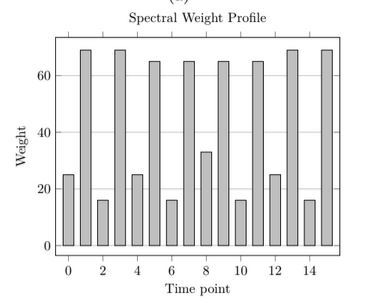
\includegraphics[width=\linewidth]{IMAGES/IMA4.JPG}
        \caption{Spectral weight profile of syncopated "Twinkle, Twinkle Little Star"}
        \label{fig:ima4}
    \end{subfigure}

    \caption{Visualisation of metric weight analysis \cite{Bemman2024}}
    \label{fig:ima_all}
\end{figure}

\section{Implementation of control} \label{section:addingcontrol}
Methods of enabling control in generative models can be split into four approaches. 1: Choice of architecture, 2: training data, 3: fine-tuning, and 4: post-hoc guidance. In table \ref{table:bigtable} we list a selection of recent symbolic deep-learning music generators with their corresponding architectures and datasets. Since deep learning models are often probabilistic, the control mechanisms are as well. They do not guarantee that the output has certain characteristics, but they \textit{condition} the probabilities of the outputs so that the outputs are more likely to have certain characteristics. 

\subsection{Control through architecture}
The choice of architecture lends itself to different types of control/conditioning. Transformers are the next-token predictors that predict based on the prior sequence. The default training paradigm allows for control with a user-defined sequence. This is true for both audio-based models such as MusicGen \cite{copet2023simple}, Jukebox \cite{Dhariwal_Jun_Payne_Kim_Radford_Sutskever_2020} and MusicLM \cite{Agostinelli_Denk_Borsos_Engel_Verzetti_Caillon_Huang_Jansen_Roberts_Tagliasacchi_et_al._2023} as well as symbolic music models such as MMT \cite{Dong_Chen_MMT_Kirkpatrick_2023}, MusicTransformer \cite{Huang_Vaswani_Uszkoreit_Shazeer_Simon_Hawthorne_Dai_Hoffman_Dinculescu_Eck_2018} and MusicBERT \cite{Zeng_Tan_Wang_MUSICBERT_2021}. Diffusion models are quite flexible compared to transformers. One can use the same model for inpainting, continuation, and - depending on the representation - melody and accompaniment generation through masking.\cite{Min_Jiang_Xia_Zhao_polyffusion_2023}\cite{Rombach_Blattmann_Lorenz_Esser_Ommer_2022}Transformers on the other hand are explicitly trained for these tasks. 

\subsection{Control through training data}
Joint training of a model with the desired control is the most common and robust method of enabling control in a generative model. MusicGen\cite{copet2023simple}, a recent text-to-music (audio) transformer is trained on 20000 hours of licensed music from Shutterstock and pond5 \footnote{https://www.shutterstock.com/music and https://www.pond5.com/} which includes textual descriptions and tags for genre, tempo, and other factors such as instrumentation. Control is achieved through the joint training of a text description and music. An example description is provided below: 

\textit{Inspirational dramatic background music! Perfect for trailer, background, advertising, historical film, movie about superheroes, teaser and many other projects!}\footnote{ https://www.pond5.com/royalty-free-music/item/95908062-inspiring-dramatic-epic-background-cinematic-music
}

Text-based control, while user-friendly and accessible to non-musicians, is inherently vague. Levels of detail and choice of words vary widely by dataset, even with standardized tags included, such as genre and tempo. This is also true of specialized music-text datasets such as MusicCaps \cite{Agostinelli_Denk_Borsos_Engel_Verzetti_Caillon_Huang_Jansen_Roberts_Tagliasacchi_et_al._2023},\cite{Lee_Doh_Jeong_2023_subjectivity_musiccaps}. For this reason, the creators of MusicGen \cite{copet2023simple} add melody conditioning alongside text conditioning and train their model jointly with the chromagram of the melody alongside the text. 

In MusicGenStyle \cite{Rouard_Adi_Copet_Roebel_Défossez_musicgenstyle_2024} the authors utilize classifier-free guidance to add style conditioning to MusicGen. They train a music-style encoder that transforms a random subsample of a given reference audio track into style tokens. The style tokens are combined with the embeddings of the text description and provided as prefixes to the model. The conditioner and the MusicGen transformer are trained jointly on the entire dataset. 
The creators of FIGARO \cite{Rütte_figaro_2023} enable time-varying control over instrumentation, note density, average pitch, and volume on a bar-by-bar basis, in a symbolic music generator through joint conditioning  of music and the selection of desired features while training. 
\subsection{Adding control through fine-tuning}

Both the melody conditioning of MusicGen \cite{copet2023simple} and the style conditioning of MusicGenStyle \cite{Rouard_Adi_Copet_Roebel_Défossez_musicgenstyle_2024} retrain the full MusicGen model on the entire dataset which comes at considerable cost. Fine-tuning or transfer learning is another method through which models are (re)-trained, but at a considerably smaller cost and using less data. Fine-tuning is widely used in the language domain to adjust large language models for niche use cases where the available data may not be sufficient to train a large model from scratch. In the examples of MusicGen and MusicGenStyle, the availability of data was not a limiting factor. The controlling elements, melody, and style, are inferred from the training data. However, fine-tuning may achieve additional control at a lower cost. 

MusiConGen \cite{Lan_Hsiao_Cheng_Yang_musicongen_2024} is a fine-tuned variation of MusicGen, which adds control for rhythm and chords. They propose the jump-finetuning mechanism, where the original model, with 1.5 Billion parameters and 48 self-attention layers, is split into blocks consisting of 4 self-attention layers. They refine the first layer of each block, freezing the remaining layers. Additionally, they apply adaptive in-attention to the first nine blocks: The output of a transformer layer is augmented with copies of the original condition. As a result, only a quarter of the original parameters are tunable, which enables training on consumer GPUs on just 250 hours of music sourced from YouTube (as opposed to 20000 hours).  In Coco-Mula \cite{Lin_cocomulla_2024}, the authors adjust a LLAMA adapter with just 4\% of parameters, keeping all original MusicGen parameters frozen and training only the adapter on a small dataset of 300 songs to add drum and chord conditioning. 

MuseBarControl \cite{Shu_Xu_Musebarcontrol_2024} is a fine-tuned version of MuseCoco \cite{Lu_Xu_Kang_Yu_Xing_Tan_Bian_MuseCoco_2023} which extends the global controls with time-varying bar level control for music-generation. They compare several approaches. In the first, they augment the prompt (which is generated from text) with additional tokens for bar-wise control of chords and adjust the loss function to incorporate that.  In the second approach, they introduce two novel methods. First, they pre-adapt the new parameters (introduced by the Lora adapter) to a separate classification task, an auxiliary task. The model classifies whether the section of music corresponds with the control tokens. The classification head added to the model for this task is removed after training. In the third step, they introduce counterfactual loss to reinforce the model's attention to the control, by rewarding the difference in negative log-likelihood between an output with the original and an output with a changed attribute. They find that combining the three strategies, pre-adaptation on a separate task followed by counterfactual loss and prompt augmentation yields the strongest model. 

\subsection{Adding control through guidance}
Other methods do not involve any fine-tuning or retraining of the original model. Adding control with additional model inputs does require at least some amount of retraining, which is not always feasible, and adding many types of control may deteriorate the model's performance. In these cases, guidance can be used to steer the model towards a certain output.
In SMITIN \cite{Koo_Wichern_Germain_SMITIN_2024} the authors intervene at inference time, while the trained model is generating, to guide MusicGen\cite{copet2023simple}  towards a certain goal. They explore guidance for ensuring the presence of certain instruments (piano/drums/bass/guitar) and to increase the quality/realism of the generated audio. For this,  the authors train linear probes that learn to associate the state of each transformer layer in the network with the goal (i.e. drums being present in the output). Then the model is steered in the direction of the probe, which increases the probability of the desired quality (drums) being present in the generated music. Guidance of transformer models has been explored in other contexts \cite{language_guide_rutte_2024}, i.e. influencing truthfulness, humor, and appropriateness, with mixed results. 

In Diffusion models, the output is sampled over several steps. At each of these steps, it is possible to intervene with guidance to direct the sampling towards a specified goal. Huang et al. \cite{Huang_rule_diffusion_2024}, repeat each sampling stage several times, and choose the output that follows a set of rules most closely. ControlNet \cite{Zhang_Rao_Agrawala_2023} adds spatial control to image generators, allowing the guidance of image generation using sketches, poses, edges, and depth maps without retraining. MusicControlNet \cite{Wu_Donahue_musicontrolnet_2023} adapts this approach to music generation, adding control for time-varying features, such as melody, dynamics, and rhythm. 

\section{Evaluation} \label{section:evaluation}
How to evaluate generated music is still an open research question. There are no generally approved methods of establishing the quality of generated music.\cite{Yin_Reuben_Stepney_Collins_2023}. However, there are several common frameworks used to evaluate music. Music generation literature often distinguishes between objective and subjective evaluation. Despite what the name suggests, objective evaluation of generated music does not measure the aesthetic quality or beauty of the music. Instead, it encompasses automated, statistical methods of analyzing and comparing generated music to human-composed music. Subjective evaluation encompasses evaluation methods that center human judgment. 

\subsection{Subjective Evaluation}
For subjective approaches, the methods vary widely \cite{Xiong_Wang_ai_eval_methods_2023}. There are simple Turing-type tests that examine whether human listeners can distinguish between generated and human-written music. There are tournament-style surveys, where different musical pieces obtained by different methods (human-written vs computer-generated) compete against each other. The listeners repeatedly select their preferred piece.\cite{Huang_Vaswani_Uszkoreit_Shazeer_Simon_Hawthorne_Dai_Hoffman_Dinculescu_Eck_2018}\cite{Rütte_figaro_2023}
Another typical approach is using (Likert) ratings along different dimensions to separate different qualities of the music. \cite{Dong_Chen_MMT_Kirkpatrick_2023}, \cite{Yu_Lu_Wang_Hu_Tan_Ye_Zhang_museformer_2022} and \cite{Chen_Smith_Spijkervet_Wang_Zou_Li_Kong_Du_2024} collect Likert ratings on coherence, richness, arrangement and consistency. In \cite{Dong_Chen_MMT_Kirkpatrick_2023}, this takes the following form: \\
Coherence: Is [the music] temporally coherent? Is the rhythm steady? Are there many out-of-context notes?;
Richness: Is [the music] rich and diverse in musical textures? Are there any repetitions and variations? Is [the music] too boring?; 
Arrangement: Are the instruments used reasonably? Are the instruments arranged properly?; \\
The specific questions asked vary with the aims of the project: 
In \cite{Yin_Reuben_Stepney_Collins_2023}, Likert ratings are collected along the dimensions of stylistic success, aesthetic pleasure, repetition, melody, harmony, and rhythm. Here, the questions for stylistic success are relevant due to their use of generative models to produce music in a certain style, specifically classical string quartets, and classical piano improvisations. 
These evaluations are often paired with statistical hypothesis testing to investigate relationships between the various ratings of the model outputs. An example would be: \textit{There is no difference between ModelA and ModelB on ratings of stylistic success}. Or \textit{ratings of melodic success are positively correlated with ratings of aesthetic pleasure}.
Finally, there are expert evaluations (which can also include Likert ratings) but also detailed analyses or even performances of the produced music \cite{Sturm_Ben-Tal_2016} \cite{Yin_Reuben_Stepney_Collins_2023}. \\

\subsection{Objective Evaluation}

Objective evaluation of generated music includes model-specific metrics and different comparative statistical metrics evaluating the outputs in comparison to other data. \cite{Xiong_Wang_ai_eval_methods_2023}. Model-specific metrics are generic evaluations of a model's success to approximate training data, these will vary depending on the model and are not indicative of stylistic success. Examples of this are Negative Log Likelihood \cite{Huang_Vaswani_Uszkoreit_Shazeer_Simon_Hawthorne_Dai_Hoffman_Dinculescu_Eck_2018} or Perplexity\cite{Rütte_figaro_2023}. 
More generally applicable are statistical investigations of the outputs, in comparison with other datasets. Measuring similarity in music is an ongoing field of research \cite{Gurjar_Moon_similarity_2018} for a large variety of different use cases, such as music retrieval, cover, genre, and artist detection. A popular comparative metric is calculating the Kulback Leibler (KL) divergence between two datasets with respect to certain features, such as the count of intervals or unique pitch classes. However to obtain the KL divergence one has to select specific features that may only capture a subset of the desired properties. Similar issues arise with other distance metrics i.e. cosine similarity, earth movers distance, or maximum overlapping area. 

Especially in the audio domain, additional AI models are often used for evaluation. MusicGen \cite{copet2023simple} uses additional classifiers to generate labels for the music and calculates the KL divergence between the generated labels. Additionally, they calculate the Frachet Audio distance, a measure devised to calculate the plausibility of audio (for music enhancement purposes) compared to a large set of studio recordings\cite{Kilgour_Frachet_2019}. Finally, they use the CLAP score which compares the corresponding text description to the latent representation of the generated audio, with the text description of the generated audio with the reference audio. \cite{Elizalde_Deshmukh_Ismail_Wang_2023}

